\documentclass[11pt]{article}  
\usepackage[spanish]{babel} 
\usepackage[utf8]{inputenc} 
\usepackage{graphicx} % Incluir imágenes en LaTeX
\usepackage{color} % Para colorear texto
\usepackage{subfigure} % Subfiguras
\usepackage{float} %Posicionamiento [h] en figuras
\usepackage{anysize} % Para personalizar el ancho de  los márgenes
\usepackage{multirow} % Para las tablas
\usepackage{listings}
\usepackage{dirtytalk}
\usepackage{mathtools}
\usepackage{amsmath}
\usepackage{enumitem}
\usepackage{amssymb}
\usepackage{verbatim}
\usepackage[T1]{fontenc} % Para el pipe
\usepackage{booktabs}
\usepackage{tikz}
\usepackage{longtable}
\usetikzlibrary{shapes,arrows}


\usepackage{listings}
\usepackage{color}

\definecolor{miverde}{rgb}{0,0.6,0}
\definecolor{migris}{rgb}{0.5,0.5,0.5}
\definecolor{mimalva}{rgb}{0.58,0,0.82}

\marginsize{3cm}{3cm}{2cm}{2cm} % Izquierda, derecha, arriba, abajo

\lstset{basicstyle=\ttfamily}
\newcommand{\lcb}{\tt {\char '173}}
\newcommand{\rcb}{\tt {\char '175}}


% Para que las referencias sean hipervínculos a las figuras o ecuaciones y
% aparezcan en colorhttps://www.overleaf.com/project/5be73eeafdbce4745a25b792
\usepackage[colorlinks=true,plainpages=true,citecolor=blue,linkcolor=blue]{hyperref}

% Para agregar encabezado y pie de página
\usepackage{fancyhdr} 
\pagestyle{fancy}
\fancyhf{}
\fancyhead[L]{\footnotesize Facultad de Ciencias} % Encabezado izquierda
\fancyhead[R]{\footnotesize UNAM}   % Encabezado derecha
\fancyfoot[C]{\thepage}  % Pie centro
\fancyfoot[L]{\footnotesize Criptografía y Seguridad}  % Pie izquierda
\renewcommand{\footrulewidth}{0.4pt} % Linea horizontal

\newcommand{\HRule}{\rule{\linewidth}{0.5mm}}

\title{FCiencias}

% ----------------------------- Termina Preámbulo ---------------------------- %

\begin{document}

% ---------------------------------- PORTADA --------------------------------- %

    \begin{center}
        \begin{minipage}{0.48\textwidth} \begin{flushleft}
        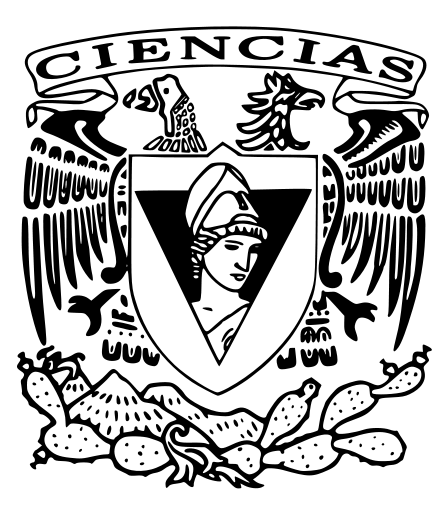
\includegraphics[scale = 0.18]{Imagenes/cnc.png}
        \end{flushleft}\end{minipage}
        \begin{minipage}{0.48\textwidth} \begin{flushright}
        
\includegraphics[scale = 0.25]{Imagenes/nam.png}
        \end{flushright}\end{minipage}

        \vspace*{-2cm}

        \textsc{\huge Universidad Nacional \\Autónoma de México}\\[1.5cm]

        \textsc{\LARGE Facultad de Ciencias}\\[3cm]

        \vspace*{1.5cm}

        \HRule \\[0.7cm]
        {\huge \bfseries Tarea 1 - Criptografía y Seguridad}\\[0.4cm]
        \HRule \\[1.5cm]

        \vfill

        \begin{minipage}{0.46\textwidth}
            \begin{center} \large
                \emph{Alumnos:}\\
                Arteaga Hernández Alejandro Iabin\\
                Martínez Ríos Ricardo\\
                Semenov Flores Dimitri
            \end{center}
        \end{minipage}
        %%% % [No quitar] - Espacio para alinear a la izquierda a los asesores %
        \begin{minipage}{0.52\textwidth}
            \begin{center} \large
                \emph{Profesor:} \\
                Galaviz Casas José de Jesús\\
                \emph{\\Ayudante:}\\ 
                Arroyo Munguía Edgar Omar\\
                \emph{\\Ayudante de Laboratorio:}\\ 
                González Vargas Andrea Itzel\\
            \end{center}
        \end{minipage}
        \vspace*{1cm}

        \vspace{2cm}
        \begin{center}
            {\large 24 de Marzo de 2019}
        \end{center}                                                             
    \end{center}

    \newpage
    
    \allowdisplaybreaks
    
    \section*{1. Demuestra lo siguiente:}
        \begin{enumerate}[label=\alph*)]
            \item \textit{Hola k ase}
            
            Supongamos que existe otro $ m' \in \mathcal{M} $ tal que $ m' \neq m $ y $ Enc_{k}(m') = c $, esto implica que la función de cifrado produce el mismo criptotexto (usando la misma llave) con dos mensajes claros diferentes.
            
            Lo anterior hace que la función de cifrado $ Enc $ no sea inyectiva y que no haya una forma de \textit{regreso} fiable (descifrado), esto es que $ \#\mathcal{M} \neq \#\mathcal{C} $, una contradicción, por lo que nuestra suposición inicial es errónea...
            
            $ \therefore \text{Para cualquier llave } k \in \mathcal{K} \text{ y } c \in \mathcal{C} \text{, existe un único } m \in \mathcal{M} \text{ tal que } Enc_{k}(m) = c $
            
            \item \textit{Sea $ S_{m,c} = \{k \in \mathcal{K}\ |\ Enc_{k}(m) = c\} $, es decir el conjunto de llaves que cifran $ m $ en $ c $. Demuestra que para distintos $ c $ y $ c' $, se tiene que $ S_{m, c} \cap S_{m, c'} = \emptyset $}
            
            Probando la contrapositiva, esto es: Si $ S_{m, c} \cap S_{m, c'} \neq \emptyset $ entonces $ c = c' $
            
            Supongamos que $ S_{m, c} \cap S_{m, c'} \neq \emptyset $, entonces sea $ k' \in  S_{m, c} \cap S_{m, c'} $
            
            Tenemos que $ Enc_{k'}(m) = c $ y $ Enc_{k'}(m) = c' $, igualando:
            
            $ c = Enc_{k'}(m) = c' \Rightarrow c = c' $
            
            $ \therefore S_{m, c} \cap S_{m, c'} \neq \emptyset \rightarrow c = c'$
            
            $ \therefore c \neq c' \rightarrow S_{m, c} \cap S_{m, c'} = \emptyset $
            
        \end{enumerate}
    
    
    
    
    \section*{2. Alicia y Bartolo escogen un espacio de claves de $\mathcal{K}$ que contiene $2^{56}$ claves. Supón que Eva tiene una computadora que puede revisar $10^{10}$ claves por segundo.}
    
    
        \begin{enumerate}[label=\alph*)]
            \item ¿Cuantos días le tomaría a Eva revisar todas las claves de $\mathcal{K}$?
            
            Tenemos que Eva puede revisar $10^{10}$ claves por segundo, vemos que $10 = 5\cdot 2 \implies 10^{10} = 5^{10} \cdot 2^{10}$
            
            Como el espacio de claves es de tamaño $2^{56}$ tenemos que la cantidad de segundos que tardaría Eva en revisar todas las claves es:
            
            \begin{equation}
                \frac{2^{56}}{10^{10}} = \frac{2^{56}}{5^{10} \cdot 2^{10}} = \frac{2^{46}}{5^{10}} = \frac{2^{10}}{5^{10}} \cdot 2^{36} = \frac{70368744177664}{9765625} \approx 7205759\ldotp40379
            \end{equation}
            
            Como $60$ segundos equivalen a un minuto y $60$ minutos equivalen a una hora tenemos que Eva tardaría la siguiente cantidad de horas, considerando que $60 = 2^2 \cdot 15$
            
            \begin{equation}
                \frac{2^{10}}{5^{10}} \cdot \frac{2^{36}}{2^4 \cdot 15^2} = \frac{2^{10}}{5^{10}} \cdot \frac{2^{32}}{15^2} \approx 2001\ldotp599834
            \end{equation}
            
            Como un día tiene $24$ horas tenemos que Eva se tardaría la siguiente cantidad de días:
            
            \begin{equation}
                \frac{2^{10}}{5^{10}} \cdot \frac{2^{32}}{2^3 \cdot 3 \cdot 15^2} = \frac{2^{10}}{5^{10}} \cdot \frac{2^{30}}{3 \cdot 15^2} = \frac{2^{10}}{5^{12}} \cdot \frac{2^{30}}{3^3}  \approx 83\ldotp39999309945
            \end{equation}
            
            \item Si Alicia t Bartolo cambian su esquema por uno con un conjunto mas grande, con $2^{B}$ claves, ¿que tan grande debe ser $B$ para que la computadora de Eva tarde 100 años revisando todas las claves? (Puedes suponer que un año tiene $365.25$ días.)
            
            Bajo la suposición de que un año tiene $365.25$ días buscamos que:
            
            \begin{equation}
                \frac{2^B}{10^{10} \cdot 2^7 \cdot 15^2 \cdot 3 \cdot 365\ldotp25} = 100 \implies 100 (10^{10} \cdot 2^7 \cdot 15^2 \cdot 3 \cdot 365\ldotp25) = 2^B
            \end{equation}
            
            Si llamamos $10^{10} \cdot 2^7 \cdot 15^2 \cdot 3 \cdot 365\ldotp25 = A$ tenemos lo siguiente:
            
            \begin{equation}
                B = \log_2(A) \implies B \approx 64\ldotp774621
            \end{equation}
            
            Por lo que necesitaríamos que $B \approx 64$.$774621$ para que Eva se tardara $100$ años
            
        \end{enumerate}
    
    
    
    
     \section*{3. Combina las siguientes parejas de ńumeros usando la operacíon de XOR a nivel de bits.\\
a) Cadenas de bits: 1100110010, 0100010001.\\
b) Ńumeros decimales: 8191, 16383.\\
c) Cadenas de bytes: 0x23ab873f, 0x1a003dfb. (Los śımbolos 0x solo son para indicar que es
hexadecimal.)}

\begin{enumerate}[label=\alph*)]
    \item 
     
        \begin{tabular}{ccccccccccc}
       & 1 & 1 & 0 & 0 & 1 & 1 & 0 & 0 & 1 & 0 \\
\oplus & 0 & 1 & 0 & 0 & 0 & 1 & 0 & 0 & 0 & 1  \\
\hline
       & 1 & 0 & 0 & 0 & 1 & 0 & 0 & 0 & 1 & 1  \\
\end{tabular}
        \item
        El número 8191 en base 2 es 1111111111111  13 unos\\
        El número 16383 en base 2 es 11111111111111 14 unos\\
      
        
         \begin{tabular}{ccccccccccccccc}
        & 0 & 1 &1 & 1 & 1 & 1 & 1 & 1 & 1 & 1 & 1 & 1 & 1 & 1 \\
\oplus  & 1 & 1 &1 & 1 & 1 & 1 & 1 & 1 & 1 & 1 & 1 & 1 & 1 & 1  \\
\hline
        & 1 & 0 &0 & 0 & 0 & 0 & 0 & 0 & 0 & 0 & 0 & 0 & 0 & 0  \\
\end{tabular}
          \item 
        El número 0x23ab873f en base 2 es 100011101010111000011100111111\\
        El número 0x1a003dfb en base 2 es 11010000000000011110111111011\\\\
       \begin{tabular}{ccccccccccccccc}
        & 100011101010111000011100111111 \\
\oplus  & 011010000000000011110111111011  \\
\hline
        & 111001101010111011101011000100  \\
\end{tabular}
\end{enumerate}
        
    \section*{4. ¿Los siguientes esquemas de cifrado son perfectamente seguros? Explica.}
    
        \begin{enumerate}[label=\alph*)]
            \item \textit{Los mensajes claros son $ \mathcal{M} = \{0, 1, \dots, 9\} $. El algoritmo 'Gen' devuelve una llave al azar del conjunto $ \mathcal{K} = \{0, 1, \dots, 13\} $. La función $ Enc_{k}(m) $ calcula $ (k + m) \mod{10} $, y $ Dec_{k}(c) $ devuelve $ (c - k) \mod{10} $}
            
            Recordando que un esquema de cifrado $ (Gen, Enc, Dec) $ sobre un espacio de mensajes $ M $ es perfectamente seguro si por cada distribución de probabilidad sobre $ M $, todo $ m \in \mathcal{M} $ y $ c \in \mathcal{C} $ donde $ Pr(C = c) > 0 $, tenemos que:
            $$ Pr(M = m\ |\ C = c) = Pr(M = m) $$
            
            Entonces la probabilidad de elegir un mensaje claro es: $ Pr(M=m) = \frac{1}{10} $, pues se escoge una valor arbitrario de $ M $. 
            
            Por otro lado, para todo $ c \in \mathcal{C} $ tenemos:
            
            $$ \displaystyle Pr(C = c) = \sum_{k, c \in Enc_k(m)} Pr(K = k) \times Pr(M = Dec_{k}(c)) $$
            
            Por lo que:
            
            $$ Pr(C = c\ |\ M = m) = \sum_{k, m \in Dec_k(c)} Pr(K = k) $$
            
            Entonces usando el teorema de Bayes:
            
            $$ \displaystyle Pr(M = m\ |\ C = c) = \frac{Pr(C = c\ |\ M = m) \times Pr(M = m)}{Pr(C = c)} $$
            
            $$ \displaystyle Pr(M = m\ |\ C = c) = \frac{Pr(M = m) \times \sum_{k, m \in Dec_k(c)} Pr(K = k)}{\sum_{k, c \in Enc_k(m)} Pr(K = k) \times Pr(M = Dec_{k}(c))} $$
            
            Supongamos que nuestro mensaje es $ 6 $ y nuestro criptotexto es $ 7 $ las llaves que producen ese criptotexto son $ 1 $ y $ 11 $, entonces tenemos que:
            
            $$ Pr(C = c\ |\ M = m) = \frac{1}{14} + \frac{1}{14} $$
            
            $$ Pr(C = c) = 2 \times \frac{1}{14} \times \frac{1}{10} = \frac{2}{140} $$
            
            Entonces: 
            
            $$ \displaystyle Pr(M = m\ |\ C = c) = \frac{\frac{2}{14} \times \frac{1}{10}}{\frac{2}{140}} = 1 $$
            
            Por lo que: 
            
            $$ \displaystyle Pr(M = m\ |\ C = c) \neq Pr(M = m) $$
            
            $ \therefore \text{El esquema no es perfectamente seguro.} $
            
            \item \textit{$ \mathcal{M} = \{m \in \{0, 1\}^{l}\ |\ \text{el último bit de m es 0}\} $. 'Gen' escoge una llave aleatoria de $ \{0,1\}^{l-1} $. $ Enc_{k}(m) $ devuelve $ m \oplus (k\ ||\ 0) $, y para $ Dec_{k}(c) $ devuelve $ c \oplus (k\ ||\ 0) $.}
            
            Este esquema siempre trabaja con mensajes claros que terminan en $ 0 $, cuando se manda a cifrar, se utiliza una llave compuesta que también tiene un $ 0 $ al final, pues la llave original tiene un bit menos que el mensaje claro, pero se le concatena uno (el $ 0 $) al entrar a la función.
            
            Lo mismo pasa en la función de descifrado, y dado que $ 0\ \oplus\ 0 = 0 $, no cambia el último bit del mensaje claro en ningún momento.
            
            \textit{One-Time Pad} tiene definidas sus funciones de cifrado y descifrado de esta manera: $ Enc_{k}(m) = m \oplus k $ y $ Dec_{k}(c) = c \oplus k $, y sus campos $ \mathcal{M}, \mathcal{C}, \mathcal{K} = \{0,1\}^{l} $
            
            Claramente estamos hablando de \textit{One-Time Pad} solo que restringido en sus campos $ \mathcal{M}, \mathcal{C} $ y $ \mathcal{K} $ (compuestas), pues todos son iguales a $ \{x \in \{0,1\}^{l}\ |\ \text{el último bit de x es 0}\} $, y sabemos que \textit{One-Time Pad} es perfectamente seguro...
            
            $ \therefore \text{El esquema es perfectamente seguro.} $
            
            \item \textit{El algoritmo de desplazamiento para mensajes de tamaño uno sobre el alfabeto ABC...Z de 26 letras.}
            
            Veamos que $ \mathcal{M} = \mathcal{C} = \mathcal{K} = \{A, B, \dots, Z\}$, entonces tenemos que $ \#\mathcal{M} = \#\mathcal{C} = \#\mathcal{K} $, por lo que podemos apoyarnos en el teorema de Shannon.
            
            En primer lugar tenemos que para toda $ k \in \mathcal{K} $, la probabilidad de elegirla para el esquema de cifrado es $ \frac{1}{26} $, lo que cumple la primera condición del teorema de que toda llave tiene una probabilidad igual de ser elegida por \textit{Gen}.
            
            En segundo lugar, sea $ I(x) $ la función que nos regresa el índice de $ x $ en el alfabeto, supongamos que existen $ k, k' \in \mathcal{K} $ (diferentes), tal que $ Enc_{k}(m) = c = Enc_{k'}(m) $, esto nos dice que:
            
            $ (I(m) + I(k)) \mod{26} = (I(m) + I(k')) \mod{26} \Rightarrow I(k) = I(k') $, pero no hay dos letras que compartan el mismo índice en el alfabeto, por lo que llegamos a una contradicción.
            
            Entonces no existen dos llaves que nos lleven al mismo criptotexto con el mismo mensaje como entrada, por lo que para cada $ m \in \mathcal{M} $ y cada $ c \in \mathcal{C} $ existe una única llave tal que $ Enc_{k}(m) = c $, lo que cumple la segunda condición del teorema de Shannon.
            
            $ \therefore \text{El esquema es perfectamente seguro.} $
            
        \end{enumerate}
        
        
        
        
        \section*{5. Sea $\Pi$ el esquema de Vigenere, donde $\mathcal{M} = \{0,,1,\dots,9\}^3$, la clave se genera escogiendo aleatoriamente un número $t \in \{1,2,3\}$ y luego se escoge una clave aleatoria de tamaño $t$.
        Un adversario $\mathcal{A}$ entrega $m_0 = aab$ y  $m_1 = abb$. Cuando se le da un texto cifrado $c = c_1 c_2 c_3$, devuelve $0$ si $c_1 = c_2$ y $1$ en caso contrario. Calcula $Pr[PrivK_{\mathcal{A},\Pi} = 1]$}
        
        Tenemos que el espacio esta restringido a mensajes de longitud 3. La clave se genera escogiendo uniformemente un $t \in \{1,2,3\}$ y luego una cadena aleatoria de longitud $t$
        
        Dado que el adversario crea y entrega los mensajes $m_0 = aab$ y $m_1 = abb$ y después recibe $c = c_1 c_2 c_3$. Si $c_1 = c_2$ devuelve $0$, en otro caso $1$ tenemos lo siguiente
        
        \begin{equation}
            Pr[PrivK_{\mathcal{A},\Pi} = 1] = (\frac{1}{2}) Pr[PrivK_{\mathcal{A},\Pi} = 1 \mid b = 0] +  (\frac{1}{2}) Pr[PrivK_{\mathcal{A},\Pi} = 1 \mid b = 1]
        \end{equation}
        
        Pero lo anterior tenemos que es 
        
        \begin{equation}
            (\frac{1}{2}) Pr[\mathcal{A} \text{ devuelve } 0\mid b = 0] +  (\frac{1}{2}) Pr[\mathcal{A} \text{ devuelve } 1\mid b = 1] 
        \end{equation}
        
        (Donde $b$ es el bit que determina si encripto $m_0$ o $m_1$
        
        Tenemos que $\mathcal{A}$ devuelve $0$ cuando en $c = c_1 c_2 c_3$ sucede que $c_1 = c_2$, si $b = 0$ entonces se cifro $m_0$ y tenemos $3$ formas de que $\mathcal{A}$ devuelva $0$
        
        \begin{itemize}
            \item Se escogió $t = 1$, por lo que la llave es de una letra que se repita para cifrar todo el mensaje. Esto solo depende de $t$ y como $t$ puede tomar $3$ valores con una distribución uniforme tenemos que lo anterior ocurre con una probabilidad de $\frac{1}{3}$
            
            \item Se escogió $t = 2$, por lo que se necesita haber escogido una clave con dos letras iguales, $t$ se escoge con una probabilidad de $\frac{1}{3}$ y dado que hay $26$ claves con dos letras iguales en el espacio de $26^2$ claves tenemos que la probabilidad de elegir una clave con dos letras iguales es $\frac{26}{26^2} = \frac{1}{26}$
            
            Por lo que lo anterior ocurre con probabilidad $\frac{1}{3} \cdot \frac{1}{26}$
            
            
            \item Se escogió $t = 3$, por lo que necesitamos haber escogido una clave con las primeras dos letras iguales. Dado que hay $26^3$ posibles claves de longitud $3$ y como hay $26$ claves de longitud $2$ con dos letras iguales y como la ultima letra que se puede elegir de $26$ formas distintas no importa tenemos que hay $26^2$ claves de longitud $3$ con las primeras dos letras iguales, por lo que la probabilidad de elegir una clave de este tipo es $\frac{26^2}{26^3} = \frac{1}{26}$ y como la probabilidad de elegir $t = 3$ es de $\frac{1}{3}$ tenemos que lo anterior ocurre con probabilidad $\frac{1}{3} \cdot \frac{1}{26}$
        \end{itemize}
        
        Dado lo anterior se da que $ Pr[\mathcal{A} \text{ devuelve } 0\mid b = 0] = \frac{1}{3} + \frac{1}{3} \frac{1}{26} + \frac{1}{3} \frac{1}{26} = \frac{1}{3} + \frac{2}{3 \cdot 26} = \frac{28}{3 \cdot 26}$
        
        
        Para calcular $Pr[PrivK_{\mathcal{A},\Pi} = 1 \mid b = 1]$ calculamos $ 1 - Pr[PrivK_{\mathcal{A},\Pi} = 0 \mid b = 1]$
        
        Como $b = 1$ entonces se escogió el mensaje $m_1 = abb$ y para que $\mathcal{A}$ devuelva $0$ tenemos los siguientes casos:
        
        \begin{itemize}
            \item Con $t = 1$ como $a$ y $b$ se cifran con la misma letra tenemos que $c_1 \neq c_2$, por lo que la probabilidad de que $\mathcal{A}$ devuelva $0$ es $0$
            
            \item Con $t = 2$, como $c_1 = c_2$ tenemos que la segunda letra de la clave vale uno mas (es la siguiente en el alfabeto) que la primera y como tenemos $26$ claves de este tipo tenemos que la probabilidad de lo anterior es  $\frac{1}{3} \cdot \frac{26}{26^2} = \frac{1}{3} \cdot \frac{1}{26}$
            
            
            \item Con $t = 3$, sucede lo mismo que con $t = 2$ y como no nos importa la ultima letra de la clave tenemos $26^2$ posibles claves, por lo que lo anterior sucede con probabilidad $\frac{1}{3} \cdot \frac{26^2}{26^3} = \frac{1}{3} \cdot \frac{1}{26}$
        \end{itemize}
        
        Por lo anterior tenemos que 
        
        \begin{align*}
            Pr[PrivK_{\mathcal{A},\Pi} = 1 \mid b = 1] &= 1 - Pr[PrivK_{\mathcal{A},\Pi} = 0 \mid b = 1]\\ 
            &= 1 - \frac{1}{3} \cdot \frac{1}{26} - \frac{1}{3} \cdot \frac{1}{26}\\
            &= 1 - \frac{2}{3 \cdot 26} = \frac{3\cdot 26 - 2}{3 \cdot 26} \\
            &= \frac{78 - 2}{78} \\
            &= \frac{76}{78}
        \end{align*}
        
        Dado esto reescribimos la expresión original
        
         \begin{equation}
            Pr[PrivK_{\mathcal{A},\Pi} = 1] = (\frac{1}{2}) \frac{28}{78} +  (\frac{1}{2})\frac{76}{78} = \frac{28}{156} + \frac{76}{156} = \frac{104}{156} = \frac{2}{3} = 0.\Bar{6}
        \end{equation}
        
        
        
        
        
        
        
        
         \section*{6. Considera el criptosistema de sustitucíon monoalfab́etica con los siguientes cambios:  $ M = C =
ALF^{l}$, es decir, los mensajes son cadenas de tamãno $l$ sobre el alfabeto ALF, y K = $P^{l}$, donde $P$ es el conjunto de permutaciones de ALF, es decir, una llave $k = k1, . . . , k`$ corresponde a 
permutaciones de ALF. La funcíon de cifrado se define como \\
$Enc_{k}(m) = k_1(m_1),k_2(m_2),...,k_l(m_l)$ donde\\ $m = m_1,m_2,...,m_l$,  $k = k_1,k_2,...,k_l$\\
a) ¿Cómo se define $Dec_k(c)$\\
b) Demuestra que el criptosistema es perfectamente seguro
}
\begin{enumerate}[label=\alph*)]
    \item Como cada elemento de k es una permutación diferente y tenemos l permutaciones diferentes,
    $c_i = k_i(m_i)$, Este criptosistema no es simétrico, ya que no se puede desencriptar de usando el mismo algoritmo. Para desencriptar tenemos $c_i$ y hay que buscar esa letra en $k_i$ y en la posición en la que se encuentre esa letra es la letra desencriptada, si $K_i(c_i)$ está en la posición 1, la letra desencriptada es A, si está en la posición 2 es L y si está en la posición 3 es F, esto para cada $K_i(c_i)$, de esa manera obtenemos el mensaje desencriptado.
    \item 
    Para demostrar que es criptograficamente seguro hay que demostrar que para cualquier criptograma $C$ ese puede ser mapeado con cualquier mensaje y con una clave k
    
    Fijamos l y suponemos que tenemos un criptograma C y un mensaje cualquiera M, y supondremos que no existe K tal que $Enc_k(M) = C$ osea que no existe $K_1(M_1),K_2(M_2),...,K_l(M_l) = C_1,C_2,...,C_l$ para que esto no suceda, al menos existe una $K_i(M_i) != C_i$, pero esto significaría, que en el conjunto de llaves no existe la permutación, que lleve de de $M_i$ a $C_i$, y esto es falso, porque ese conjunto de llaves, por definición tiene todas las posibles permutaciones, y esto es contradicción, entonces nuestra suposición de que  $Enc_k(M) = C$ no existe es FALSA.
    Entonces  $Enc_k(M) = C$ existe\\
    Todas las claves son equiprobables, porque en el conjunto de llaves están todas las permutaciones, y como es un conjunto, están sin repetición, entonces las llaves son únicas en el conjunto y eso las hace equiprobables.\\
    Por último, \\PD la cardinalidad de los conjuntos de llaves, mensajes y criptogramas son iguales. \\\\
    La definición del conjunto de llaves, es el conjunto de combinaciones, de las permutaciones de tamaño l, como hay 3 elementos las permutaciones por cada letra son 3, ya que hay 3 opciones de codificación por letra, puede ser A,L o F, entonces tenemos $3^l$ claves que encriptan a criptogramas diferentes, que es la cardinalidad de mensajes,\\
    como todo criptograma es obtenible con una clave k y cualquier mensaje, entonces hay,al menos tantos criptogramas como mensajes, pero como cada criptograma es a la vez un mensaje válido y cada mensaje es un criptograma válido, entonces estos 2 conjuntos tienen la misma cardinalidad.
    
    y el sistema es criptográficamente seguro.
    
    Y esto tiene sentido, ya que cada criptograma es obtenible con el mismo número de claves, por lo que probabilidad de cada criptograma es la misma de ser obtenida, con una llave k y un mensaje M
\end{enumerate}
         
        \section*{7. Definimos $ \Pi $ como una versión modificada de \textit{One-Time Pad}, donde $ \mathcal{M} = \{0, 1\}^{l}$, pero ahora $ \mathcal{K} $ son las cadenas de $ l $ bits con un número par de unos; el cifrado y el descifrado son iguales a los originales. Construye un adversario $ \mathcal{A} $ tal que $ Pr(PrivK_{\mathcal{A}, \Pi} = 1) = 1 $ }
        
        Sean:
        $$ P_{1} = \{x \in \{0, 1\}^{l}\ |\ \text{cadena de l-bits con número par de unos}\} $$
        $$ I_{1} = \{y \in \{0, 1\}^{l}\ |\ \text{cadena de l-bits con número impar de unos}\} $$\\
        Con $ p,q \in P_{1} $ y $ r,s \in I_{1} $, XOR cumple lo siguiente:
        
        \begin{itemize}
            \item $ (p \oplus q) \in P_{1} $
            \item $ (p \oplus r) \in I_{1} $
            \item $ (r \oplus s) \in P_{1} $
        \end{itemize}
        
        El adversario $ \mathcal{A} $ utilizara esto para tener éxito, en primer lugar sus mensajes de salida serán: $ m_{0} y m_{1} $ tal que $ m_{0} \in P_{1} $ y $ m_{1} \in I_{1} $ (uno con una cantidad par de unos y el otro con una cantidad impar de unos).\\
        
        Sea $ c_{x} $ el criptotexto que recibe el adversario de regreso al cifrarse alguno de los 2 mensajes (con ayuda del bit $ b $), como $ c_{x} = m_{b} \oplus k $ (con $ k \in P_{1} $), lo siguiente que hace $ \mathcal{A} $ es contar el numero de unos en $ c_{x} $ y su bit de salida $  b' $ esta definido de esta forma:
        
        \begin{equation*}
        b' =
            \begin{cases}
            0    & \text{Si } c_{x} \in P_{1},\ (m_{b} \oplus k), k \in P_{1} \rightarrow m_{b} = m_{0}\\
            1    & \text{Si } c_{x} \in I_{1},\ (m_{b} \oplus k) \in I_{1} \text{ y } k \in P_{1} \rightarrow m_{b} = m_{1}
            \end{cases}
        \end{equation*}
        
        Por las propiedades antes mencionadas, $ \mathcal{A} $ siempre sabrá cual de los dos mensajes fue cifrado al contar el número de unos de $ c_{x} $.\\
        
        $ \therefore Pr(PrivK_{\mathcal{A}, \Pi} = 1) = 1 $ 
        
        
        
        \section*{8. Sea $\Pi$ un esquema de cifrado perfectamente seguro con un espacio de llaves $\mathcal{K} = \{0,1\}\l$. Supongamos que un banco desea partir una llave $k$ en tres partes $p_1 , p_2 , p_3$ de forma que para poder descifrar es necesario usar dos de las tres partes. De esta forma, cada parte se le entrega a un ejecutivo distinto, y el descifrado solo es posible si se juntan al menos dos de los tres ejecutivos.}
        
        
        Inicialmente el banco genera aleatoriamente dos pares de llaves $(k_1, k_{1}')$ y $(k_2.k_{2}')$ que satisfacen las relación
        \begin{center}
            $k_1 \oplus k_{1}' = k_2 \oplus k_{2}' = k$
        \end{center}
        
        y al primer ejecutivo se le asigna la parte $p_1 = (k_1 , k_2)$.
        
        \begin{enumerate}[label=\alph*)]
            \item Define las partes $p_2$ y $p_3$ para que cumpla la condición deseada, es decir, que con cualesquiera dos partes se puede recuperar $k$, pero con una sola no es posible.
            
            Dada la igualdad
            
            \begin{center}
                $k_1 \oplus k_{1}' = k_2 \oplus k_{2}' = k$
            \end{center}
            
            Recordemos que la operación $\oplus$ es conmutativa, asociativa, que $a \oplus a = 0$ y que $a \oplus 0 = a$. Dado esto 
            notemos lo siguiente
            
            \begin{align*}
                k_1 \oplus (k_1 \oplus k_{1}') &= k_1 \oplus (k_2 \oplus k_{2}') = k_1 \oplus k \\
                (k_1 \oplus k_1) \oplus k_{1}' &= (k_2 \oplus k_{2}') \oplus k_1 = k_1 \oplus k \\
                k_{1}' & = k_2 \oplus (k_{2}' \oplus k_1) = k_1 \oplus k \\
                k_2 \oplus k_{1}' & = k_2 \oplus (k_2 \oplus (k_{2}' \oplus k_1)) = k_2 \oplus (k_1 \oplus k) \\
                k_2 \oplus k_{1}' & = (k_2 \oplus k_2) \oplus (k_{2}' \oplus k_1) = k_2 \oplus (k_1 \oplus k) \\
                k_2 \oplus k_{1}' & = k_{2}' \oplus k_1 = k_2 \oplus (k_1 \oplus k)
            \end{align*}
            
            Dado lo anterior si definimos $p_2 = (k_2, k_{1}')$ y $p_3 = (k_{2}', k_1)$ tenemos que el ejecutivo con $p_2$ no puede obtener la llave $k$ por si solo y el ejecutivo con $p_3$ tampoco puede obtener la llave $k$ por si solo.
            
            Y notemos lo siguiente sobre las combinaciones de $p_1, p_2, p_3$
            
            \begin{itemize}
                \item Si juntamos $(p_1, p_2)$ tenemos la igualdad $k_1 \oplus k_{1}' = k$
                
                \item Si juntamos $(p_1, p_3)$ tenemos la igualdad $k_2 \oplus k_{2}' = k$
                
                \item Si juntamos $(p_2, p_3)$ tememos la igualdad $k_1 \oplus k_{1}' = k = k_2 \oplus k_{2}'$
            \end{itemize}
            
            \item Haz los cambios necesarios en el esquema anterior, de forma que ahora se necesiten $3$ de $5$ partes para poder descifrar. (Y con dos partes no se obtiene información sobre $k$.)
            
            Definimos tres tercias tales que cumple:
            
            \begin{center}
            $k_1 \oplus k_1' \oplus k_1'' = k_2 \oplus k_2' \oplus k_2'' = k_3 \oplus k_3' \oplus k_3'' = k$
            
            \end{center}
            
                
            Dado esto proponemos las partes $p_1 = (k_1', k_2'',k_3), p_2 = (k_1'', k_2, k_3'), p_3 = (k_1, k_2', k_3''), p_4 = (k_1, k_2'',k_3'), p_5 = (k_1', k_2,k_3'')$
            
            
            Definimos las categorías $0,1$ y $2$ que corresponden a la cantidad de $'$ que tiene. Notemos que cada parte tiene un elemento de cada categoría, cada entrada tiene un índice distinto y que un elemento $k_i$ aparece a lo más en dos partes, también vemos que si tomamos la pareja de partes tales que el elemento $k_i$ es el mismo entonces las otras dos parejas de elementos son de distinta categoría
            
            Dado lo anterior tenemos que si tomamos dos parejas $p_i,p_j$ entonces a lo más solo un $k_i$ podrá ser igual y habrá dos parejas $k_j$ de distinta categoría entre ellos y además de categoría distinta a $k_i$, por lo que solo nos faltara un
            elemento de la categoría de $k_i$ para crear la llave y como solo pueden existir dos parejas tales que su entrada $k_i$ sea la misma entonces cualquier otra parte que tomemos tendrá uno de los elementos de la categoría faltante
            
            También tenemos que no damos información demás sobre la llave ya que a lo mas tenemos dos elementos de la igualdad descrita
            
            
        \end{enumerate}
        
        
        
        
        
        
        
        
        
        \section*{9.Considera el siguiente escenario sobre una votación. Se tienen t votantes, y cada uno puede votar
0 o 1. Al final de la votacíon una persona anuncia el resultado S, que corresponde a la suma de
todos los votos. Para llevar a cabo la votacíon de forma que ninǵun votante sepa nada m ́as que el
resultado S, se propone el siguiente protocolo.\\
\\
Sea n > t un entero. Al inicio de la votacíon el encargado genera $c_0 <= $\{0, 1, . . . n−1\}. El primer
votante recibe $c_0$ y obtiene $c1 = c0 + v1$ ḿod $n$, donde $v_1 \in \{0, 1\} $ es su voto. Luego le pasa
$c_1$ al votante 2 y este hace lo ańalogo. Sucesivamente, el votante i recibe el valor $c_{i−1}$, calcula
$c_i = c_{i−1} + v_i$ mod n  y se lo entrega al votante i + 1. El votante t obtiene $c_t$ y se lo entrega al
encargado, este último calcula  $ S = c_t-c_0$ mod $n$ y lo anuncia a todos los votantes.
\\\\
a) Muestra que el encargado al final efectivamente calcula la suma de todos los votos.\\\\
b) Suponiendo que en el protocolo los votantes se comportan honestamente, al final de la votacíon
cada votante i solo es capaz de conocer S y el valor $c_{i−1}$ (adeḿas del propio voto $v_i$\\
definimos $Vista_i = (S, c_{i − 1})$. Si fijamos los valores de i y S, el votante i puede tener distintas vistas
$Vista_i$ ,dependiendo de ćomo fueron los votos de los de ́as votantes.
¿Los diferentes valores posibles de $Vista_i$ sirven para que el votante i pueda distinguir el voto
de otro votante? ¿Por qúe?\\
\\
c) Suṕon que dos votantes deshonestos quieren conocer el voto de un tercero. ¿Ćomo pueden lograrlo? (Sin usar el ḿetodo del garrote.)}

\begin{enumerate}[label=\alph*)]
\item Sea S la suma de todos los votos y $S'= C_t - C_0 $ mod $ n$\\
Sabemos que $C_t = C_{t-1} + V_t$ mod $n$, \\por lo tanto $S'= (C_{t-1} + V_t$ mod $n) - C_0 $ mod $ n \\= S'= C_{t-1} + V_t - C_0 $ mod $ n$, si hacemos esto para todas las $C_i$ entonces\\
$S'= C_0 + V_1 +V_2+...+V_t - C_0$ mod $n$ pero la suma de todas las $V_i = S$ entonces, $S' = C_0 + S - C_0 $ mod $ n $ y por último $S'= S$ mod $ n $ Pero como $n>t$ y S a lo más es t, entonces no afecta nunca lo afectará, y no modificará a S'

\item Si,en caso donde solo fueran 2 votantes podría saber que votó el otro,  si pasara el caso en el que todos votan 1, entonces todos sabrían el voto de los demás, lo mismo si votaran 0, en caso que uno votara diferente, ese podría saber el voto de todos los demás, pero los demás no sabrían, pero para saber, en el caso en que los votos no son homogéneos, no se podría, porque para saber el voto de alguien más, necesitar saber, para el voto j-ésimo necesitas $C_j, C_{j-1},n $ aunque fueras el penúltimo, no puedes saber el siguiente voto, porque no conoces, n, en ningún otro caso, se sabría más, entonces no se puede.
\item
Se tendrían que compartir sus sumas parciales y votos, en el caso, donde fueran los votantes i e i+2, podrían saber lo que votó el votante en medio, sabiendo si se modificó la suma o no,
si la suma parcial fuera t-a y estuvieran separados a lo más a lugares, podrían saber si todos votaron 0 o todos votaron 1, tienen que ser t-a lugares porque si no se puede hacer el módulo y se pierde esa información.
En general, se necesita saber  $C_j, C_{j-1},n $ para saber el voto de alguien
\end{enumerate}
    
\end{document}